\documentclass[a4paper,titlepage, twoside]{report}
\usepackage[T1]{fontenc}
\usepackage{charter}
\usepackage[bitstream-charter]{mathdesign}
\usepackage{siunitx}
\usepackage{amsmath}
\usepackage{mathtools}
\usepackage{subcaption}
\usepackage[backend=biber, style=authoryear, firstinits=true, maxcitenames=2]{biblatex}
\usepackage{minted}
\usepackage{booktabs}

\renewbibmacro{in:}{}

\addbibresource{radiation.bib}

\newcommand\eqnumbered{\addtocounter{equation}{1}\tag{\theequation}}
\newcommand\Kdown{K\!\!\downarrow}
\newcommand\Kup{K\!\!\uparrow}
\newcommand\Ldown{L\!\!\downarrow}
\newcommand\Lup{L\!\!\uparrow}
\newcommand\Kdownsfc{{K\!\!\downarrow}_\mathrm{SFC}}
\newcommand\Kdowntoa{{K\!\!\downarrow}_\mathrm{TOA}}
\newcommand\Ldownsfc{{L\!\!\downarrow}_\mathrm{SFC}}

\begin{document}
\expandafter\def\csname PY@tok@err\endcsname{}

\title{Impact of urban atmospheric conditions on radiation receipt in London}
\author{Elizabeth Erhbar, Emily McKie, Maurice John Lally, James Shaw}
\maketitle

\begin{abstract}
TODO

A model is developed to predict downwelling longwave and shortwave radiation at the surface using observed cloud cover, air temperature and relative humidity.  Model results have a root-mean-squared error of \SI{111}{\watt\per\meter\squared} for shortwave and \SI{47}{\watt\per\meter\squared} for longwave.
\end{abstract}

\tableofcontents

\chapter{Background}
\section{The global energy budget}
The global radiation budget between the surface, atmosphere and space is shown in Figure~\ref{fig:energy-budget}.  The net radiation balance ($Q^\ast$) represents these energy exchanges within a vertical profile of the atmosphere and provides energy for atmospheric motion, heat transport and sensible fluxes \parencite{offerle}.
\begin{align}
Q^\ast = \left( \Kdown - \Kup \right) + \left( \Ldown - \Lup \right)
\end{align}

$Q^\ast$ is comprised of incoming ($\downarrow$) and outgoing ($\uparrow$) shortwave ($K$) and longwave ($L$) radiation. $\Kdown$ and downwelling $\Lup$ are the fluxes examined here, as the amount received at the surface depends on atmospheric conditions such as cloud cover and aerosols. $Q^\ast$ varies diurnally as $\Kdown$ is dominant during the day from solar radiation and $\Ldown$ has a stronger influence at night, but overall there is a net radiation balance of longwave and shortwave bands \parencite{oke}.

\begin{figure}
\centering
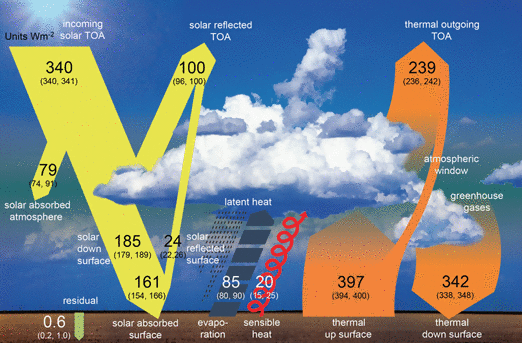
\includegraphics[width=\textwidth]{radiation.png}
\caption{The global mean radiation balance of the Earth. Arrows show the global average energy balance fluxes with their uncertainty ranges (\si{\watt\per\meter\squared}) for shortwave radiation (yellow) and longwave radiation (orange) (Source: \cite{wild})}
\label{fig:energy-budget}
\end{figure}

The radiation in the atmospheric profile is accounted for by absorption ($a$), reflection ($\alpha$) and transmittion ($t$) at a wavelength ($\lambda$) \parencite{fest}
\begin{align}
a_\lambda + \alpha_\lambda + t_\lambda = 1 \label{eq:radiation-budget}
\end{align}
The reflectivity determines outgoing radiation and depends on the albedo value, which varies with local conditions including cloud cover and land surface type. The absorptivity is the flux that is neither reflected nor transmitted (see section~\ref{sec:radiative-transfer}.  The value of each component of equation~\ref{eq:radiation-budget} is affected by atmospheric conditions, and therefore affects the amount of $\Kdown$ and $\Lup$ received at the surface. This is shown in Figure~\ref{fig:energy-budget}.

Figure~\ref{fig:energy-budget} demonstrates the energy balance fluxes on a global scale, however this report focuses on these fluxes on a local scale, within a city. The urban canyon effect increases reflectivity between buildings and lowers the sky view factor, reducing the incoming shortwave radiation receipt at the surface and the emission of longwave radiation \parencite{cleugh}.  The urban canopy also has a lower albedo, therefore less shortwave radiation is reflected at the surface.

\section{Shortwave and longwave radiation}
The incoming solar radiation at the top of the atmosphere (TOA) is determined by the solar `constant' \SI{1366}{\watt\per\meter\squared}, but this is distributed around the Earth to give the average insolation for the Earth's surface of \SI{340}{\watt\per\meter\squared} \parencite{ambaum}.  The incoming shortwave radiation flux is a function of latitude, season and time of day due to variations in the solar zenith angle and the distance of the earth from the sun \parencite{ambaum}.  The absorbed radiation is reradiated as longwave radiation.

Shortwave radiation is around the visible spectrum and shorter wavelengths, from \SIrange{0.2}{3}{\micro\meter} and peaking in the visible wavelength range from \SIrange{0.45}{0.75}{\micro\meter} \parencite{salby}.  Radiation around the thermal infrared is longwave radiation (from \SIrange{4.5}{45}{\micro\meter}).

\section{Radiative transfer}
\label{sec:radiative-transfer}
Radiation is transferred by absorption through air. For a layer of air,  the change in intensity of a beam is equal to the negative radiative intensity at that wavelength multiplied by the change in optical depth, therefore the intensity of a beam decreases with time through absorption \parencite{ambaum}.
\begin{align}
\mathrm{d}I_\lambda = - I\lambda \cdot \mathrm{d} \tau_\lambda
\end{align}
where $I$ is radiative intensity and $\tau$ is optical depth at wavelength $\lambda$.
The absorption cross-section and number density of absorbers indicates the area of the beam that will become extinct. The Beer-Lambert law relates the optical depth to the number density of absorbers, their absorption cross-section and geometric depth of the layer \parencite{ambaum}.
\begin{align}
\tau_\lambda = \tilde{n} \cdot \sigma_\lambda \cdot l
\end{align}
where $\tilde{n}$ is the number density of absorbers, $\sigma_\lambda$ is the absorbtion cross section at wavelength $\lambda$ and $l$ is the geometric depth of the layer.

This is important as atmospheric conditions, including cloud cover and aerosols, define the amount of absorbers and therefore the optical depth, which determines the amount of shortwave radiation receipt at the surface.

The radiation that is transmitted through a layer (transmittance) also depends on the wavelength. The Beer-Lambert law can be used to model attenuation by scattering---the change of direction of a beam of radiation. In clean air, most shortwave radiation is scattered by Rayleigh scattering \parencite{chameides}.

\section{Impact of the urban atmosphere}
It is important to study the impact of the urban atmosphere on radiation receipt, as cities are a good analogue for global anthropogenic climate change \parencite{cleugh}.  Increasing both cloud and aerosol optical depth leads to a reduction in incoming shortwave radiation at the surface as these particles attenuate the incoming beam, and increase longwave radiation \parencite{ipcc}.

\subsection{Cloud cover}
Shortwave radiation is separated into direct and diffuse beam, with attenuation mostly caused by cloud cover. Clouds also enhance incoming longwave radiation, particularly at nighttime \parencite{kotthaus}.  Clouds reflect and absorb incoming shortwave radiation, as well as attenuation, the amount depending on the cloud height, amount and thickness \parencite{iqbal}.  The thickness relates to the optical depth of a cloud. Using Equation~\ref{eq:radiation-budget}, it can be seen that an increase in reflectivity and absorptivity from the clouds results in decreased transmissivity to the surface. Previous observations suggest that on average of \SI{69}{\watt\per\meter\squared} of incoming solar radiation is reflected by cloud and \SI{20}{\watt\per\meter\squared} absorbed \parencite{salby}.  In addition to cloud amount, the solar zenith angle also influences the amount of attenuation from cloud cover, as it increases the length of the beam path through the cloud \parencite{oke}.  Cloud height impacts the amount of transmission, as high cloud reflects less than low cloud \parencite{liou}.

\subsection{Aerosols}
Aerosols also scatter and attenuate incoming shortwave radiation, with the effect depending on the type and density of aerosols. Aerosols are a chemical mixture of suspended solid and liquid particles, ranging in size from less than \SI{0.1}{\micro\meter} to large coarse particles; fine particles from \SIrange{0.1}{3}{\micro\meter} are typical for large scale air pollution \parencite{chameides}.  Aerosols can be natural, but around anthropogenic sources such as the burning of fossil fuel, anthropogenic aerosols are the significant source. 

Solar radiative flux is affected by aerosols directly, through the particles scattering and absorbing the incoming beam, and indirectly as they enhance the formation of cloud drops by acting as cloud condensation nuclei \parencite{chameides}.  Transmittance is altered as aerosols increase diffuse radiation and the attenuation of UV radiation \parencite{cleugh}.  The impact of the indirect effect is more difficult to quantify and so is less well understood. Aerosol optical depth increases with pollution, so that scattering and absorption from aerosols can dominate over Rayleigh scattering, for example the aerosol optical depth is 0.2-0.5 over the eastern United States \parencite{chameides}.  In urban areas there is a higher density of emissions, therefore more shortwave is made extinct before reaching the surface, resulting in a reduction of surface shortwave radiation in urban areas compared to rural areas.  Table~\ref{tab:aerosol-sw} summarises the results of previous research that quantifies this reduction in shortwave radiation due to the urban effect. Global climate models estimate the reduction in surface shortwave radiation from aerosols to be from \SIrange{1.3}{3.3}{\watt\per\meter\squared}.  At the top of the atmosphere the net radiation change is estimated to be up to \SI{-9}{\watt\per\meter\squared} over land \parencite{ipcc}.

\begin{table}
\centering
\begin{tabular}{ c c c }
\toprule
Source &	Location &	Reduction of incoming shortwave \\ \midrule
\cite{chameides} &	NE China (model) over agricultural land from regional haze & 5\% -- 30\% \\
\cite{cleugh} & 	Global &	5\% if low aerosol concentration.  Up to 30\%, e.g. Hong Kong \\
\cite{psiloglou} &	Model using data from the National Observatory in Athens & 10\% -- 20 \% \\
\cite{rouse} &		Hamilton, Canada & 10\% \\
\cite{ball} &		Eastern US & 8\% \\
\cite{ramanathan} &	Indian Ocean & \SI{-20}{\watt\per\meter\squared} (6\%) \\
\cite{ipcc} &		Global model estimate & \SIrange{-1.3}{-3.3}{\watt\per\meter\squared} (less than 1\%) \\ \bottomrule
\end{tabular}
\caption{Observed decrease in incoming shortwave radiation caused by aerosol effects from urban areas (ranked by decreasing reduction of incoming shortwave)}
\label{tab:aerosol-sw}
\end{table}

Overall, there should be little change in net radiation as there is a small increase in downward longwave radiation from aerosols, whilst incoming shortwave is reduced \parencite{ipcc}.  Longwave radiation is enhanced as urban canyons have a lower sky view factor, lessening longwave radiation loss \parencite{cleugh}.  The aerosol optical depth affects the proportion of shortwave that becomes extinct; where low aerosol conditions are reported, incoming radiation is reduced by 5\%, compared to up to 30\% for large cities such as Hong Kong \parencite{cleugh}.  It has been suggested that this decrease in surface radiation is more important in controlling the energy budget than the increase in surface temperature form greenhouse gas induced warming \parencite{liepert}.

\subsection{Precipitation}
Precipitation can cause an increase in shortwave radiation due to rainout and washout. Water vapour condenses on aerosol particles (rainout), which are then washed out by precipitation with approximately 30\% of aerosol mass in water \parencite{bourcier}.  The efficiency of aerosol removal through wet deposition depends on the intensity, duration and type of precipitation \parencite{van-leeuwen}.

\chapter{Methodology}
\section{Instruments}
A Vaisala CL31 ceilometer is used to measure cloud cover percentage and backscatter, in order to identify cloud layers and aerosols. Data were collected by King's College London every 15 minutes between October 2010 and October 2012, and can measure to 7.6 km in the vertical \parencite{vaisala}, although readings rarely get to this height. A laser beam is sent up vertically and small fractions of light are scattered by particles, some of which is directed back to the lidar receiver. Using the speed of light, the time taken for the backscatter can be converted into a spatial range. The ceilometer can identify three cloud layers and also the rate of diffusion, which can give the concentration of air pollutants. The accuracy of backscatter measurements is $\pm1\%$ \parencite{vaisala}.

The CNR4 net radiometer is used to measure the radiation fluxes of incoming and outgoing shortwave and longwave radiation. A pyranometer pair measures shortwave radiation from \SIrange{300}{2800}{\nano\meter} and a pyrgeometer pair measures longwave radiation within the spectral range from \SIrange{4500}{42000}{\nano\meter}, with an acuracy of $\pm10\%$ \parencite{kipp}.

\section{Location}
The instruments are placed on the roof of King's College London, with the measurement tower at \SI{49}{\meter} above street level \parencite{kotthaus}.  Measurement height is important within urban areas; \cite{kotthaus} show that flux processes are observed at different scales within urban areas due to differing measurement heights. At this height instruments are less affected by bias, for example from particularly heavy traffic routes, and the effect of urban canyons. The site is in central London (\ang{51.5}N, \ang{0.1}W) in the `central activities zone' \parencite{kotthaus} (Figure~\ref{fig:location}).  The surface of the building and surrounding area is primarily concrete and asphalt.

\begin{figure}
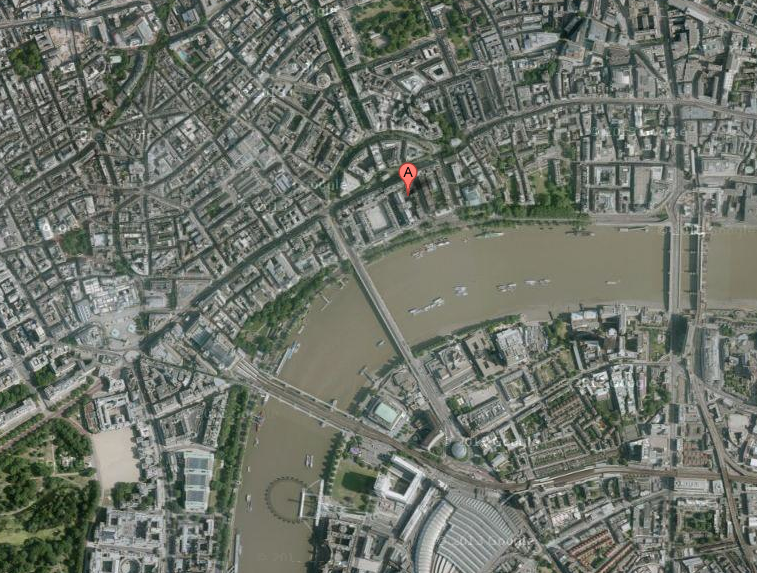
\includegraphics[width=\textwidth]{map.png}
\caption{Satellite image showing location of measurement tower in London (A) (Source: \cite{google-maps})}
\label{fig:location}
\end{figure}


\chapter{Model}
The radiation model was constructed around observation data collected from a Met mast from January 2010 to December 2012, and Vaisala CL31 cloud cover data from October to December 2010.  Both instruments were installed at KSS. TODO: footnote explaining where that is

\section{Design}
The model diagnoses shortwave and longwave radiation from three easily observed meteorological variables: air temperature near the surface, cloud cover, and relative humidity.  The shortwave radiation model is driven by the diurnal and seasonal variation of insolation through an atmosphere with an amount of cloud cover.  In section~\ref{sec:longwave-model} a simple longwave model is presented that is based on air temperature alone, which is then refined based on longwave parameterisation from \cite{loridan}.

\subsection{Geometry}
\begin{figure}
\centering
\begin{subfigure}{0.52\textwidth}
\hspace{-1em}
\input{toa-model-annual}
\caption{Annual variation of insolation in 2010.  Midday insolation peaks in the summer when $\theta$ is close to zero.}
\end{subfigure}
\hfill
\begin{subfigure}{0.4\textwidth}
\hspace{-2.2em}
\input{toa-model-daily}
\caption{Insolation on January 1 2010.  Times of day in UTC with sunrise and sunset occuring around 08:00 and 16:00 respectively.}
\end{subfigure}
\caption{Modelled insolation at top of the atmosphere ($\Kdowntoa$) above London (\SI{51}{\degree N}) showing annual and diurnal periodicity.  $\Kdowntoa$ is dependent upon the solar zenith angle $\theta$ as given by equation~\ref{eq:solar-zenith}}
\label{fig:toa-model}
\end{figure}

The model initially estimates the insolation at the top of the atmosphere (TOA).  The insolation at the top of the atmosphere, $\Kdowntoa$, is related to the total solar irradiance, $S_0$ \parencite[p. 175]{ambaum}
\begin{align}
\Kdowntoa &= S_0 \left( \langle r_E \rangle / r_E(t) \right)^2 \cos \theta
\intertext{where $\langle r_E \rangle$ is the average distance between the Earth and the Sun and $r_E(t)$ is the distance at a given time.  This orbital eccentricity is neglected since it is small, so the equation simplifies to}
\Kdowntoa &= S_0 \cos \theta
\intertext{where $\theta$ is the solar zenith angle which is given by \cite[p. 317]{jacobson}}
\cos \theta &= \sin \varphi \sin \delta + \cos \varphi \cos \delta \cos h \label{eq:solar-zenith}
\end{align}
where $\varphi$ is the latitude, $h$ is the hour angle and $\delta$ is the declination of the Sun.  Given we are concerned with radiation in London, we can assume a longitude of \ang{0}, so the hour angle is approximately \parencite[p. 319]{jacobson}
\begin{align}
h = \left( t(\mathrm{seconds}) \cdot \ang{360} / 86400 \right) - \ang{180}
\end{align}
where $t(\mathrm{seconds})$ is the number of seconds past midnight UTC.

The declination of the Sun $\delta$ is approximated by \parencite{jacobson}
\begin{align}
\delta &= \sin^{-1} \left( \sin \varepsilon_\mathrm{ob} \sin \lambda_\mathrm{ec} \right) \\
\intertext{where $\varepsilon_\mathrm{ob}$ is the obliquity of the ecliptic and $\lambda_\mathrm{ec}$ is the ecliptic longitude of the Sun.  These are approximated by \parencite{jacobson}}
\varepsilon_\mathrm{ob} &= \ang{23.439} - \ang{0.0000004} N_\mathrm{JD} \\
\lambda_\mathrm{ec} &= \ang{280.460} + \ang{0.9856474} N_\mathrm{JD} + \ang{1.915} \sin g_\mathrm{M} + \ang{0.020} \sin 2g_\mathrm{M}
\intertext{where $g_\mathrm{M}$ is the mean anomaly of the sun which is \parencite{jacobson}}
g_\mathrm{M} &= \ang{357.528} + \ang{0.9856003} N_\mathrm{JD}
\intertext{where}
N_\mathrm{JD} &= 364.5 + (Y - 2001) \times 365 + D_\mathrm{L} + D_\mathrm{J} \\
D_\mathrm{L} &= \left\{ 
  \begin{array}{l l}
    \mathrm{INT}(Y - 2001)/4 & \quad Y \geq 2001 \\
    \mathrm{INT}(Y - 2000)/4 - 1 & \quad Y < 2001
  \end{array} \right.
\end{align}
where $Y$ is the year and $D_\mathrm{J}$ is the Julian day of the year with $D_\mathrm{J}=1$ being January 1.  This model results in insolation with annual and diurnal periods as seen in Figure~\ref{fig:toa-model}.


\subsection{Shortwave insolation}
To model the insolation at the surface we estimate the optical depth of the atmosphere at a given time, $\tau(t)$.  This is calculated by comparing insolation at the surface, $\Kdownsfc$, and at the top of the atmosphere, $\Kdowntoa$ using the Beer-Lambert law \parencite{stephens}
\begin{align}
&& \Kdownsfc &= \Kdowntoa\: \exp \left( -\frac{\tau}{\mu} \right) \\
\text{or equivalently} && \tau &= \mu \: \ln \left( \frac{\Kdownsfc}{\Kdowntoa} \right)
\end{align}
The model treats optical depth as a linear function of cloud cover fraction $F_\mathrm{cloud}$ such that 
\begin{align}
\tau &= \gamma F_\mathrm{cloud} + \tau_\mathrm{clear} \label{eq:linear-sw-cloud}
\end{align}
where $\tau_\mathrm{clear}$ is the optical depth of clear sky ($F_\mathrm{cloud} = 0$) and $\gamma$ is the cloud optical depth coefficient.   Values for $\gamma$ and $\tau_\mathrm{clear}$ are found empirically in section~\ref{sec:parameterisation}.

\subsection{Longwave radiation}
\label{sec:longwave-model}
The downwelling longwave radiation at the surface, $\Ldownsfc$, can be estimated by using a single-slab, isothermal atmosphere.  Using the observed air temperature immediately above the surface and assuming the atmosphere radiates as a blackbody we can use the Stefan--Boltzmann law \parencite[p. 168]{ambaum}
\begin{align}
\Ldownsfc = \varepsilon_\mathrm{ATM} \sigma T_\mathrm{ATM}^4 \label{eq:stefan-boltzmann}
\end{align}
if we assume that the atmospheric emissivity $\varepsilon_\mathrm{ATM} = 1$.  In our analysis in section~\ref{sec:model-analysis} we find that this simple approximation overestimates downwelling longwave radiation.

\cite{loridan} propose a more refined longwave radiation model that is controlled by relative humidity $\mathrm{RH}$, cloud cover fraction $F_\mathrm{cloud}$ as well as air temperature.  Precipitable water content is a function of vapour pressure $e$ and temperature $T_\mathrm{ATM}$ \parencite{loridan}
\begin{align}
w &= 46.5 \frac{e(\si{\hecto\pascal})}{T_\mathrm{ATM}(\si{\kelvin})} \label{eq:precip-water-vapour}
\intertext{The vapour pressure is a function of relative humidity and saturated vapour pressure $e_s$ \parencite{ambaum}}
e &= \mathrm{RH} \: e_s(T)
\intertext{where the saturated vapour pressure can be estimated by Tetens' formula \parencite{ambaum}}
e_s(\si{\hecto\pascal}) &= 6.112 \exp \left( \frac{17.67 T(\si{\celsius})}{T(\si{\celsius}) + 243.5} \right)
\intertext{The atmospheric emissivity is based on clear-sky emissivity and cloud cover fraction \parencite{loridan}}
\varepsilon_\mathrm{ATM} &= \varepsilon_\mathrm{clear} + \left(1 - \varepsilon_\mathrm{clear} \right) F_\mathrm{cloud} \label{eq:emissive-atm} \\
\varepsilon_\mathrm{clear} &= 1 - \left( 1 + w \right) \exp \left( - \sqrt{1.2 + 3w} \right) \label{eq:clear-sky-emissivity}
\intertext{Substituting into Equation~\ref{eq:stefan-boltzmann}, the parameterisation of $\Ldownsfc$ becomes \parencite{loridan}}
\Ldownsfc &= \left[ \varepsilon_\mathrm{clear} + \left( 1 - \varepsilon_\mathrm{clear} \right) F_\mathrm{cloud} \right] \sigma T_\mathrm{ATM}^4 \label{eq:loridan-ldown}
\end{align}
To gain physical intuition, the absorptivity of the atmosphere increases with cloud cover and, by Kirchhoff's law \parencite[p. 166]{ambaum}, so does the emissivity $\varepsilon_\mathrm{ATM}$ (equation~\ref{eq:emissive-atm}).  In clear skies, the absorptivity increases with water vapour content since water vapour is a moderate absorber of longwave radiation.  Figure~\ref{fig:emissivity-response} shows the relation between emissivity, relative humidity and cloud cover fraction.

\begin{figure}
\centering
\begin{subfigure}{0.48\textwidth}
\input{clear-emissivity}
\caption{Emissivity response to relative humidity at $T_\mathrm{ATM}$ \SIrange{0}{20}{\celsius} in clear sky conditions from equation~\ref{eq:clear-sky-emissivity}.  Warmer temperatures cause increased absorptivity and emissivity.}
\end{subfigure}
\hfill
\begin{subfigure}{0.48\textwidth}
\input{cloud-emissivity}
\caption{Emissivity response to cloud cover at $T_\mathrm{ATM} = \SI{10}{\celsius}$ and RH from 0.5 to 1.0 given by equation~\ref{eq:emissive-atm}. Cloud cover fraction has a greater effect at lower relative humidities.}
\end{subfigure}
\caption{Emissivity responses to cloud cover and relative humidity}
\label{fig:emissivity-response}
\end{figure}

\subsection{Data cleansing}
The model must handle records with missing or nonphysical values that are present in the KSS dataset.  

Optical depth is not calculated in two cases.  First, for some records, the observed $\Kdownsfc$ is greater than the calculated $\Kdowntoa$.  This typically occurs at night when $\Kdowntoa$ is always zero but, due to instrument error, $\Kdownsfc$ is a small non-zero value.  Second, optical depth is effectively infinite when $\Kdownsfc = 0$ so it is not calculated.

At times when cloud coverage observations are unavailable this affects modelled shortwave and longwave radiation.  Surface insolation is modelled using the mean optical depth $\langle \tau \rangle$.  Cloud cover is assumed to be zero in the Loridan longwave model.

\section{Parameterisation}
\label{sec:parameterisation}

\begin{figure}
\centering
\input{cloud-tau-fit}
\caption{Relation between cloud cover and observed optical depth.  For the KSS dataset shown, 3085 records exist for which both cloud cover and optical depth are present.  In the majority of readings no cloud cover or full cloud cover was observed.  The spread of optical depths is significantly larger at times of full cloud cover.}
\label{fig:cloud-tau-fit}
\end{figure}

In Figure~\ref{fig:cloud-tau-fit} we find a weak relationship between observed cloud cover fraction $F_\mathrm{cloud}$ and optical depth $\tau$.  Using a simple linear regression we find coefficients for equation~\ref{eq:linear-sw-cloud} where $\tau_\mathrm{clear} = 0.14$ and $\gamma =  0.29$.

After data cleansing, the average optical depth was found to be $\langle \tau \rangle = 0.45$.  The value is only used twice since, in the KSS dataset, there are only two records without cloud coverage data.

Coefficients for precipitable water content $w$ and clear sky emissivity $\varepsilon_\mathrm{clear}$ were taken directly from \cite{loridan} (see equations~\ref{eq:precip-water-vapour} and \ref{eq:clear-sky-emissivity} respectively).  In \cite{loridan}, cloud cover is approximated from relative humidity and air temperature values.  However, since the CL31 dataset contains precomputed cloud coverage values, we use these in model calculations.

\section{Analysis}
\label{sec:model-analysis}
The model was evaluated by comparing its output with radiation observed at KSS.  Longwave radiation is better approximated but overestimates the observed value.  

As seen in Figure~\ref{fig:shortwave-verification}, the model diagnoses shortwave radiation with cloud cover observations alone with a root-mean-square error (RMSE) of \SI{111}{\watt\per\meter\squared}.  Since $R^2 = 0.2$ for the linear regression between cloud cover and optical depth, this error should be expected.

When total cloud cover is observed for an extended duration of about one day, shortwave radiation is overestimated.  An example is shown in Figure~\ref{fig:extended-cloud}.  In section~\ref{sec:further-work} we suggest a way of improving this.

\begin{table}
\centering
\begin{tabular}{ r @{\hspace{2em}} c c c c }
\toprule
Longwave model &	RMSE (\si{\watt\per\square\meter}) &	$\langle \Ldownsfc^\mathrm{model} - \Ldownsfc^\mathrm{obs} \rangle$ (\si{\watt\per\square\meter}) \\ \midrule
Temperature-only &	59 &	 				\num[retain-explicit-plus]{+47} \\
Loridan &		47 &					\num{-32} \\ \bottomrule
\end{tabular}
\caption{Summary of longwave model errors.  $\langle \Ldownsfc^\mathrm{model} - \Ldownsfc^\mathrm{obs} \rangle$ the mean difference between all model and observed values.  The Loridan model has lower RMSE and has a mean is closer to the observed mean.}
\label{tab:longwave-error}
\end{table}

Longwave radiation is systematically overestimated by the simple temperature-only model.  This is clearly seen in Figure~\ref{fig:longwave-verification}.  The simple longwave model has a RMSE of \SI{59}{\watt\per\meter\squared}.  The Loridan longwave model is more accurate having a RMSE of \SI{47}{\watt\per\meter\squared}.  The two longwave model errors are summarized in Table~\ref{tab:longwave-error}.

When $F_\mathrm{cloud} = 1$, both models give the same overestimated result.  Recall that, in the Loridan model, $\Ldownsfc = \left[ \varepsilon_\mathrm{clear} + \left( 1 - \varepsilon_\mathrm{clear} \right) F_\mathrm{cloud} \right] \sigma T_\mathrm{ATM}^4$ (equation~\ref{eq:loridan-ldown}) which simplifies to $\Ldownsfc = \sigma T_\mathrm{ATM}^4$ in total cloud cover.  By comparing the average difference between all model and observation values we find that both models overestimate by \SI{12}{\watt\per\square\meter} when $F_\mathrm{cloud} = 1$.  We return to this issue in section~\ref{sec:further-work}.

There are several possibilities for model error in longwave radiation.  First, both models assume an isothermal atmosphere and use air temperature at the surface to estimate $\Ldownsfc$.  They both assume that air radiates as a black body.  Second, aerosol concentration is not included in either model; possible aerosol effects are discussed in section~\ref{sec:further-work}.  Third, recalculating the coefficients for the Loridan model using on the KSS dataset may reduce model error (see equations~\ref{eq:precip-water-vapour} and \ref{eq:clear-sky-emissivity}).
\begin {figure}
\centering
\input{shortwave-verification}
\caption{Comparison of modelled and observed shortwave radiation from October 23 -- October 25, 2010.  Cloud cover varied over October 23 affecting $\Kdownsfc$.  Cloud cover was minimal on October 24.  There were clear skies across London on October 25 so $\Kdownsfc \approx \varepsilon_\mathrm{clear} \Kdowntoa$.}
\label{fig:shortwave-verification}
\end{figure}

\begin{figure}
\centering
\input{extended-cloud}
\caption{Modelled and observed shortwave radiation with extended cloud cover from October 13 -- October 15, 2010.  The model overestimates $\Kdownsfc$ on all three days.}
\label{fig:extended-cloud}
\end{figure}

\begin{figure}
\centering
\input{longwave-verification}
\caption{Modelled and observed longwave radiation from October 27 -- October 29, 2010.  The temperature-only model overestimates $\Ldownsfc$ by \SI{10}{\watt\per\meter\squared} to \SI{100}{\watt\per\meter\squared}.  It is seen that the Loridan model better captures variation in longwave radiation.}
\label{fig:longwave-verification}
\end{figure}

\section{Further work}
\label{sec:further-work}
Our analysis has neglected observation error and uncertainty in cloud optical depth coefficient $\gamma$.  Ideally, our model would incorporate these sources of error and model radiation as a probability distribution rather than a single value.

The shortwave model presented is a crude one.  A selection of superior cloud cover shortwave models are described in \cite{ingram}.  The shortwave model could also be improved by including rayleigh scattering, water vapour and aerosol extinction effects.

In our analysis we found that the Loridan model overestimates $\Ldownsfc$ during total cloud cover.  It should be possible to rescale equation~\ref{eq:loridan-ldown} so that $\Ldownsfc<\sigma T_\mathrm{ATM}^4$ for any amount of cloud.

Additionally, it may be worthwhile exploring the rainfall measurements present in the KSS dataset since precipitation is known to reduce aerosol concentrations due to washout \parencite{loosmore}.

\printbibliography

\appendix
\chapter{Model source code}
Source code is available online at \url{https://github.com/hertzsprung/urban-radiation}.

\section{\texttt{radiation.py}}
\inputminted[fontsize=\footnotesize, tabsize=4]{python}{radiation.py}

\section{\texttt{one\_year\_toa.py}}
\inputminted[fontsize=\footnotesize, tabsize=4]{python}{one_year_toa.py}

\section{\texttt{model\_obs\_merge.py}}
\inputminted[fontsize=\footnotesize, tabsize=4]{python}{model_obs_merge.py}

\end{document}
